\chapter{Explaining Neural Networks}

% This section covers intro to explainablity of neural networks.
% We define aims and scope of explainability
% Why do we want to be able to explain models.
% some legal criterions
% some paper about patholigists not really believing the network. 
% We discuss utilized methods.

This chapter covers introduction to the growing field of explainable artificial intelligence. We start with short overview of the field itself, following by motivation for understanding decisions of neural networks, alongside overview of legal obligations placed on decision support systems by European Union. We continue with overview of several explainability methods, suitable for our domain and task. This will serve as a foundation for the next chapter, where we evaluate selected methods against our benchmark.

In the contemporary literature, several terms are used when addressing the incomprehensibility of ML models. Arrieta et al. distinguish following idioms []:
% TODO - make actual definitions

\begin{enumerate}
    \item Understandability: Characteristic of a model to make a human understand its function without any need for explaining its internal structure or the algorithmic means by which the model processes data internally
    \item Comprehensibility: Ability of a learning algorithm to represent its learned knowledge in a human understandable fashion 
    \item Interpretability: Ability to explain or to provide the meaning in understandable terms to a human.
    \item Explainability: An accurate proxy of the decision maker and comprehensible to humans.
    \item Transparency: A model is considered to be transparent if by itself it is understandable.
\end{enumerate}

They further emphasize the distinction between interpretability and explainability -- interpretability, closely coupled with transparency are inherent and passive characteristics of a machine learning model. On the contrary, explainability is an initiated action taken to clarify model's internal details . Both can be seen as means to achieve understandability -- how a human can make sense of decisions made by the model [].

% https://pdf.sciencedirectassets.com/272144/1-s2.0-S1566253519X0007X/1-s2.0-S1566253519308103/main.pdf


\section{Need for understandability}

State of the art neural network models are often products of billions of parameters []. A term "black-box" models has been coined, to highlight their complex internal mechanics. In a crusade for ever-better performance and accuracy, models inherently grow in size and depth. Increasing size and complexity raises concerns of research community and general public, whether these networks can be trusted and used responsibly. [] []

% https://pdf.sciencedirectassets.com/272144/1-s2.0-S1566253519X0007X/1-s2.0-S1566253519308103/main.pdf
% https://ieeexplore.ieee.org/document/8400040

\subsection*{Spurious Correlations}
% systematic bias & reserch
Distrust does not stem only from lack of insight into model's internal reasoning. In certain cases, seemingly flawless performance of machine learning models may in fact be a result of a systematic bias in training and evaluation data. Commonly used example is an experiment by Ribeiro et al. where they purposely trained a logistic regression classifier to distinguish between wolves and husky dogs. The dataset was compiled such that images of wolves consistently featured snow in the background, whereas those of huskies did not. This led the classifier to base its decisions on the presence of snow in the picture, rather of the animal itself []. 

% husky - https://arxiv.org/pdf/1602.04938.pdf

A more naturally occurring example is presented in Figure \ref{fig:horse-tag}. One can see, that a \emph{capable} model may arrive at the desired output, despite that it disregards features, on which people would base their decision-making process. 

Instances such as these demonstrate that the understandability of a decision support system isn't just an issue for the end-user. It's also advantageous for the model's development cycle. Gaining insights into the factors influencing the model's decisions allows us to responsibly evaluate if its reasoning aligns with our expectations -- and take according measures if not.


\begin{figure}[!h]
    \begin{center}
    \begin{minipage}{1\textwidth}
      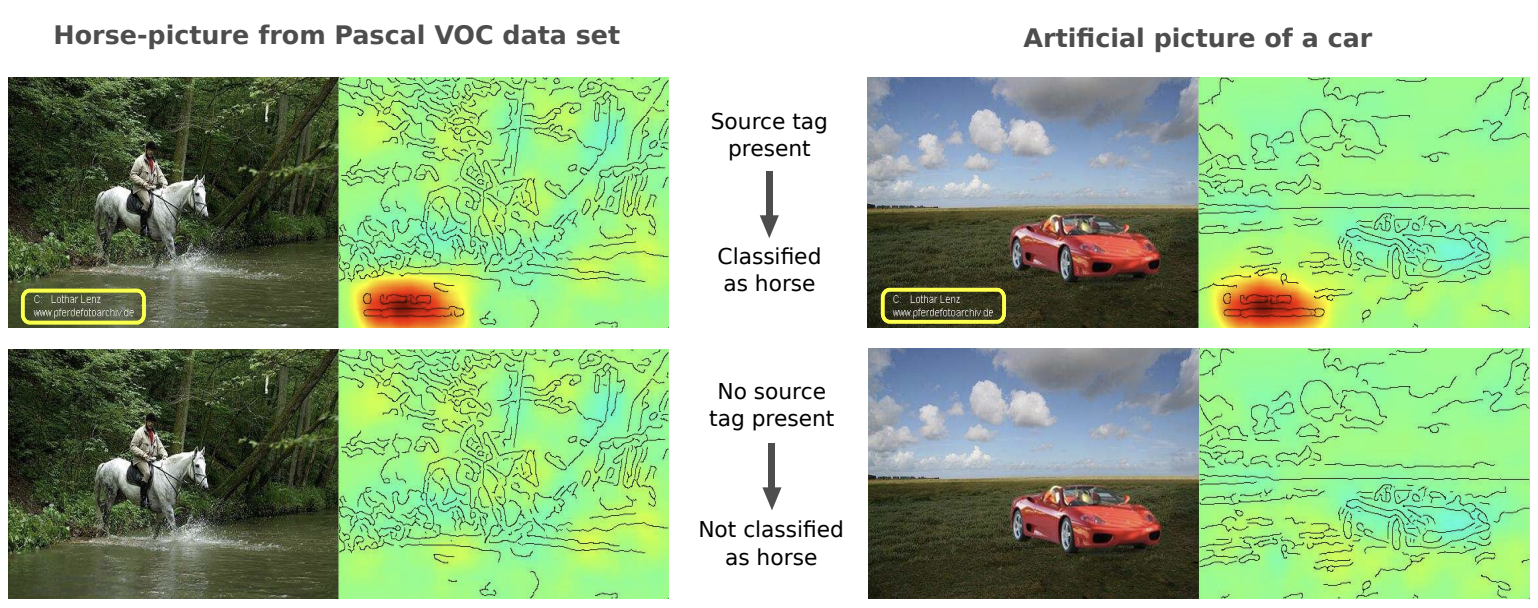
\includegraphics[width=\textwidth]{img/horse-tag.png}
    \end{minipage}
    \caption{Experiment conducted by Samek et al []. Model was trained on PASCAL-VOC dataset []. After the training, they found presence of so-called \emph{spurious correlation}. Pictures of horses are classified solely on whether the bottom-left corner of an input image contains a source tag. If the source tag manually added to an otherwise correctly classified image of a car -- the model changes its prediction, and the image is classified as a horse instead.}
    \label{fig:horse-tag}
    \end{center}

\end{figure}

% horse - https://arxiv.org/pdf/1902.10178.pdf

% medicine pov
\subsection*{Explainability in medical domain}

Such spurious correlations and the black-box tag lead clinicians to be sceptic about integrating AI in healthcare. Recent survey by GE HealthCare concludes, that out of 2000 clinicians participating in the survey, $58$ percent does not have overall trust in AI systems and $44$ percent of respondents believe, that the AI-based systems are biased []. Achieving trust of both clinicians and patients is crucial in order to achieve industry-wide utilization of machine learning-based systems.

% https://www.gehealthcare.com/about/newsroom/press-releases/ge-healthcare-reimagining-better-health-study-identifies-the-barriers-to-achieving-a-more-human-and-flexible-healthcare-experience

% legal
\subsection*{Legal obligations for AI explainability in the European Union}

Given certain applications, understanding the model is not only a moral obligation. In 2016, the European Union included what is often referred to as the \emph{right to explanation} within the General Data Protection Regulation (GDPR). Specifically, Articles 13 and 14 give individuals the right to receive 'meaningful information about the logic involved', when they are a part of automatic decision-making process.  This pose a challenge for industry, implicating that adequate measures need to be taken in place in order to fully integrate decision support systems based on deep learning. More on what Articles 13 and 14 mean for AI is to be found in a paper by Goodman and Flaxman [].

% https://arxiv.org/pdf/1606.08813.pdf

Another piece of legislation from the European Union is anticipated to be implemented in May or June of 2024. \emph{AI Act} introduces a series of regulations for machine learning-based AI systems. The legislation is notably more detailed and exhaustive than Articles 13 and 14 of the GDPR, yielding mixed responses from domain experts. While the full implications are yet to be seen, it already imposes several restrictions on what needs to be met before deploying machine learning models. In particular, one section specifically targets high risk AI systems and states that a 'providers must build for human oversight, incorporating ``human-machine interface tools'' to ensure systems "can be effectively overseen by natural persons"'. Several other important aspects of model's life-cycle are revised as well, ranging from training dataset to technical documentation. Comprehensive overview of the article is beyond the scope of this thesis, and is summarized by Veale and Borgesius in [].

% https://www.degruyter.com/document/doi/10.9785/cri-2021-220402/html

\section{Explainable Artificial Intelligence}

Rapid development of deep learning models and scarcity of trust among users call for tools and methods, which allow us to understand and justify outputs of otherwise opaque systems. With the aim to shed light on internal processes of machine learning models, a sub-field of Explainable Artificial Intelligence (XAI) covers a range of techniques to make models more understandable, while preserving their performance and effectiveness. XAI techniques enable humans to build trust and manage machine learning based decision support systems --- a crucial part of assimilation of systems based on deep learning [darpa?]. The exact borders of the field are not firmly set, and the notion of what does it mean to explain a model is an ongoing matter of discussion [].

\todo{find citations, forgot to write down}

Throughout this thesis, `XAI' will refer specifically to the subfield dedicated to advancing explainability in AI, while 'explainable artificial intelligence' will denote the attribute of machine learning models that enables certain level of understandability. To describe explainable artificial intelligence, Arietta et al. [] suggest to use the following definition: \emph{Given an audience, an explainable Artificial Intelligence is one that produces details or reasons to make its functioning clear or easy to understand}.\newline
% taxonomy paper

\noindent
The field of XAI distinguishes between two means, how to make artificial intelligence understandable:

\begin{enumerate}
    \item Using transparent model: Models based on linear regression or decision trees are inherently interpretable -- therefore understandable by itself. By looking at their parameters, we are able to clearly derive how they came to given conclusion.
    \item Using post-hoc explainability methods: When dealing with neural networks, we gain little insight into how they operate by simply inspecting their weights. Therefore we must implement auxiliary methods, which simplify and distill the reasoning of networks, so that according to the definition -- we get a clear and easy to understand explanation. Post-hoc explainability methods can be further divided into two subgroups -- global methods explaining model as a whole and local methods, focused on internal reasoning behind prediction for particular input sample.
\end{enumerate}

In the recent years, plethora of both global and local post-hoc explainability methods has been introduced in order to help grasp decision process of deep neural networks []. Post-hoc methods can be further divided into two groups. Model-specific methods are designed to explain only models with specific features and capabilities -- such as attention-based models or convolutional neural networks. On the contrary, model-agnostic methods can be used to explain arbitrary machine learning model.

% https://pdf.sciencedirectassets.com/272144/1-s2.0-S1566253519X0007X/1-s2.0-S1566253519308103/main.pdf
\section{Making CNN's Understandable}

For convolutional neural networks, industry-wide standard is to visually highlight parts of a image, which are considered \emph{important} to the model. The result of such visualization is commonly referred to as a \emph{saliency map}, class activation map or attribution map. There is no consensus on terminology, and we will use the term saliency map to describe any heatmap that identifies features considered significant by a post-hoc method. 

\todo{highlight, that we use explainability methods to achieve understandability}

\noindent
In following subsections we overview several explainability methods we will later benchmark in Chapter 4. We deliberately chose methods, which were not covered in previous work by RationAI's team. Popular methods such as LIME, Deconvolution or ...  were either computationaly too expensive, or produced sub-par results, which are not deemed satisfactory []. We rather focused on methods used specifically created for explaining CNNs, leveraging their ability of spatial memory.

\todo{cite matej and vojta}

\todo{ref chapter}

\subsection{Occlusion}

Occlusion is model-agnostic method and comes from family of so-called input perturbation based methods. Occlusion computes attribution map by systematically covering square parts in input image and observing the change in models prediction confidence on the perturbed image. Intuitively, we expect that when we cover (occlude) important part of the input image, the confidence of our classifier drops. In contrary, when we cover region which does not contain any important features, the output should not differ too much from output for the non-perturbed image. Visual example can be seen in Figure \ref{fig:occ-saliency}. This approach gives us a rough heatmap of input feature saliency.

Experiment conducted by Gallo et al. [] shows, that in the domain of prostate cancer detection, this method produces semantically correct saliency maps. Occlusion detects several recognized Gleason patterns, \todo{vytiahnut z matejovho clanku, ze ktore}. Sadly, occlusion comes with high computational complexity and resource utilization. For our use-case, explaining a single tile of $512px \times 512px$, the method needs 289 forward passes to compute the attribution map. On a machine with $8$ cores, $16$GB of RAM and $48$GB of GPU memory capacity, occlusion needs approx. $2$ seconds and $40$GB of GPU memory to generate single saliency map. Recall Section Y and processing WSI. In our test set, slide size varies from 400 to 4000 tiles per slide. Omitting auxiliary saliency map processing, this method takes anywhere from $13$ to $130$ minutes to explain a single WSI.
% https://pdf.sciencedirectassets.com/277035/1-s2.0-S1871678423X00065/1-s2.0-S1871678423000511/main.pdf

\begin{figure}[!h]
    \begin{center}
    \begin{minipage}{1\textwidth}
      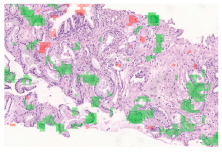
\includegraphics[width=\textwidth]{img/occ-saliency.png}
    \end{minipage}
    \caption{Sample of prostate tissue with occlusion generated saliency. Green areas denote parts important for the model, while red parts signify areas which are not pro-cancerous. Since saliency maps are generated on a tile-level, they are further composed and overlapping areas averaged to produce slide-level saliency map. Sigmoid function is applied to saliency maps before combining, as is reported in [gallo] to have positive effect on smoothing and stability of the explanations.}
    \label{fig:occ-saliency}
    \end{center}
\end{figure}

\todo{Better image :)}

\subsection{CAM}

Zhout et al. show, that introducing GAP layer to a convolutional neural network has a welcome side-effect -- aside of regularization during training, it enhances networks localization capabilities, despite being trained on image-level labels only -- without specifying, where in the input the object of interest resides. Their proposed method, called Class Activation Mapping (CAM) is used to visually highlight regions of input image used by the CNN to make its prediction for certain class $c$. This method is model-specific, since it works only with networks having GAP (or GMP) as intermediate layer between the last convolutional layer and final fully-connected layer []. 
% https://arxiv.org/pdf/1512.04150.pdf

On intuitive level, CAM is simply weighted sum activations of the last convolutional layer. To formalize, consider a network with convolutional layer $L$ with $F$ activation maps $A^1, A^2, ..., A^F$, followed by GAP layer and single fully-connected layer. In the FC layer, we fix neuron denoting class $c$, for which we want to compute a saliency map. Recall Equation ..., and that GAP reduces value of each activation map $A^k$ to a single value $a^k$ --- average of the activations. The score of network for class $c$ is then calculated...
\begin{equation}
    y^c = \sum_{k=1}^F w_{ck}  a^k.
\end{equation}

To construct class activation map for class $c$, we reverse-engineer calculation of $y^c$. The saliency map is constructed out of individual mappings, and mapping for spatial element $S^c_{xy}$ is calculated as a weighted sum of activation maps $A^k$
\begin{equation}
    S^c = \sum_{k=1}^F w_{ck}  A^k.
\end{equation}
To obtain saliency map $S^c_{\text{CAM}}$, we simply calculate mappings for all pairs $x, y$. Mass of $S^c_{CAM}$ is equal to the score $s^c$ and directly indicates importance of the respective spatial locations. If pooling layers are present in the network, they lead to activations of $L$ having smaller dimension than the input. This is addressed by up-sampling the $S^c_{CAM}$ to the size of original input image.
\medskip


Authors point out, that this method is particularly useful for networks with GAP layer. They believe that using GMP leads to the method pointing out to the single most discriminatory location, instead of all of them as it is case for GAP. While this has been largely confirmed by their experiment on ILSVRC dataset [], we believe that the method is worth considering for our use case. Models employed in the experiment are trained to distinguish between $1000$ classes, with their last convolutional layer having $1024$ units. This configuration suggests a roughly one-to-one relationship between the activations produced by the network and the classes it aims to identify. In our setting, the last convolutional layer has $512$ units --- we posit that even though we only extract the most discriminative location from each activation map, having 512 units should still yield robust localization performance.

\subsection{GradCAM++}

GradCAM++ is popular gradient-based model-specific method used to spatially attribute convolutional layer features with respect to a given class, leveraging gradients flowing in the network. It improves upon its successful predecessor GradCAM []. We first overview the GradCAM methods in order to see its limitations and how GradCAM++ specifically targets them.\newline

% https://arxiv.org/pdf/1610.02391.pdf

\noindent
GradCAM stands for Gradient-Weighted Class Activation Maps. Unlike CAM, GradCAM is capable of explaining various CNN architectures, without necessary for a global pooling layer. The idea is, that since convolutional layer holds spatial information about its activations --- we can highlight the important ones using partial derivatives with respect to the score $y^c$ of class $c$.

Principle of GradCAM is fairly straightforward. Let $L$ be a fixed convolutional layer of our network with $F$ units, which activation maps are $A^1, A^2, ... A^F$, each of size $Z$. We compute importance weight $i^c_k$ for feature map $A^k$ as gradient of $y^c$ with respect to $A^k$. Individual partial derivatives are global-average-pooled, yielding following equation []:
% \todo{Why do we use raw score instead of softmaxed, if we do not perturb the image?}

\begin{equation}
    i^c_k = \frac{1}{|A^k|} \sum_{x,y} \frac{\partial y^c}{\partial\! A^k_{xy}}
\end{equation}

To obtain a coarse saliency map, we compute weighted combination of activations and their respective importance. $ReLU$ is applied over the heatmap to get only positive values advocating for important features with respect to class $c$ [].

\begin{equation}
    S^c_{GradCAM} = \operatorname{ReLU}(\sum_k i^c_k A^k)
\end{equation}
Inspiration for using $\operatorname{ReLU}$ -- therefore taking only positive partial derivatives -- comes from Deconvolution and Guided Backpropagation, both being post-hoc methods already covered by Gallo et al. in []. In case the saliency map $S^c_{GradCAM}$ is smaller than input image, we up-sample it as in the case of $S^c_{CAM}$.\newline

\noindent
Chattopadhyay and Sarkar [] built novel method on foundation of GradCAM while addressing some of its problems. They observed, that if multiple occurences of class of interest $c$ are present in the input image, localization capabilities of GradCAM worsen. According to authors, this stems from using unweighted partial derivatives in Equation ... If there are multiple occurrences of class $c$, different feature maps may get activated, resulting in diluted and faded saliency map. They proposed generalized solution, equivalent in terms of computational performance. GradCAM++ introduces weights to the computation of partial derivatives, slightly changing the Equation 3.1 into []:
%\DeclareMathOperator{\relu}{ReLU}
\begin{equation}
    i^c_k = \sum_{x,y} \alpha^{kc}_{xy} \operatorname{ReLU}(\frac{\delta Y^c}{\delta A^k_{xy}}),
\end{equation}
where $Y = \operatorname{softmax}(y)$.
\todo{GradCAM vs GradCAM++ obrazok z original paperu, tie veci co som spominal vyssie}

Thanks to additional coefficient $\alpha^{kc}_{xy}$ for partial derivatives, all instances of class $c$ will be highlighted with equal importance. Unlike GradCAM, GradCAM++ computes the partial derivative for activated score, as it needs it to be smooth function. This is denoted by $Y^c$ in Equation 3.3. For derivation of $\alpha$, visit third chapter of original GradCAM++ paper []. To obtain saliency map $S^c_{GradCAM++}$, we simply plug $i^c_k$ into Equation 3.2.

% https://arxiv.org/pdf/1710.11063.pdf

\subsection{HiResCAM}

HiResCAM is another gradient based method building upon GradCAM's success. First step is the same as for GradCAM++ --- we need to compute partial derivatives of $y^c$ with respect to activation map $A^k$. Instead of condensing importance of the activation map to a single value, we perform pair-wise multiplication of $\nabla y^c(A^k)$ and respective activation map, yielding following equation []: 

\begin{equation}
    (S^c_{\text{PHiResCAM}})_{xy}
        = \sum_k \frac{\partial y^c}{\partial A^k_{xy}} A^k_{xy}.
\end{equation}
% https://arxiv.org/pdf/2011.08891.pdf

The rationale is that such approach better reflects how models ``sees" the input image. This way, individual activations are scaled accordingly to the gradient before they are summed up to form the final saliency map. Authors of HiResCAM arrived to similar observation as in case of GradCAM, that GAP-ing the partial derivatives in Equation 3.1 leads to blurring the effect of the gradient across feature maps. 

In addition to the method itself, authors present a proof of HiResCAM's capabilities. The proof shows, that for convolutional networks ending in one fully connected layer, HiResCAM guarantees to visually highlight all parts of input image which increase class score $y^c$, given we compute the saliency map for the last convolutional layer []. Unfortunately, the proof cannot be extended as is for our model introduced in Section .... While the model ends in one fully connected layer, it is separated from the last convolutional layer by intermediate global max pooling operation, which reduces each feature map to a single value. This breaks down the assumption that we can extract spatial information from the feature maps, since such information will be destroyed in the GMP operation. 

Authors show, that given a model has CAM architecture, HiResCAM saliency collapses to produce identical results as the CAM method from Section .... However, our model is using GMP instead of GAP, therefore the theoretical implications are unclear.

\todo{Maybe it is the same :D}

\subsection{ScoreCAM}

With aim to bridge gap between perturbation-based and gradient-based methods, Wang and Wang [] introduced ScoreCAM to tackle GradCAM's flaws from different perspective. Unlike it is the case for previous CAM-based methods, ScoreCAM does not rely on partial derivatives to compute the saliency. Instead, author relies on so-called channel-wise increase in confidence, which is, given input vector $X$ and baseline vector $X_b$, defined as:

\begin{equation}
    cic^k = f\bigl(X \odot \operatorname{upscale}(A^k)\bigr) - f(X_b)
\end{equation}

Where $upsample$ is a function, which resizes activation map $A^k$ to the size of input and $scale$ is scaling function to squish up-sampled activation to range $[0, 1]$. What we get, is a score indicating how much networks confidence changes, if we only supply areas of image where filter $f^k$ found a pattern it is trained to detect. We calculate the final saliency map using channel-wise increase of confidence as our weight for convolutional layer activation maps, yielding []:

\begin{equation}
    S_{ScoreCAM}^c = ReLU\biggl(\sum_k cic^k A^k\biggr)
\end{equation}


As a result, we get rid of dependency of intermediat GAP (GMP) layer and gradient. According to the conducted experiments, ScoreCAM is able to locate multiple objects with the same activation map, something we believe might be hard to achieve due to our utilization of GMP layer --- which zeroes our all but one partial derivative for each activation map. In the original paper, authors also mention that saliency maps computed by ScoreCAM are more "focused" than the ones computed by GradCAM++. While having focused saliency maps is desired property, comparing results visually and drawing any conclusions is considered being an anectodal evidence and proper quantitative assessment needs to be done [].

% anecdotal evidence paper

\subsection{AblationCAM}


Riding the wave of gradient free methods, AblationCAM utilizes ablation analysis to compute importance of activation maps. AblationCAM computes how inidividual activation maps contribute to the final score $y^c$ by iteratively removing them and observing drop in confidence of the model. This replaces gradient, preventing gradient saturation or explosion. Influence of removal of feature map $A^k$ to final score is defined as:

\todo{Gradient saturation}

\begin{equation}
    i^c_k = \frac{y^c - y^c_k}{y^c}
\end{equation}

The idea is, that if we remove filter important to the network when assessing presence of class $c$, the score $y^c$ should drop. To obtain the final saliency map, we compute the ablation weights for layer of interest, yielding the following equation:

\begin{equation}
    L^c_{AblationCAM} = ReLU(\sum_k i^c_k A_k)
\end{equation}

As it is the case for ScoreCAM, this method does not require gradient or GAP, and therefore it should be able to detect the occurrence of multiple instances of input feature captured by single activation map.

\subsection{Layer-Wise Relevance Propagation}

While Occlusion estimated feature importance by observing changes in output and CAM-based methods utilized spatial information in convolutional layer, Layer-Wise Relevance Propagation (LRP) takes different approach. Given a output score of the network, LRP utilizes several types of propagation rules to redistribute the score from output layer all the way down to the input pixels. Idea is, that we can look at how individual features contribute to the networks output --- each feature value is weighted and sent to the upper layer across the whole network, ultimately contributing to the final class score. In reverse fashion, we can compute the input pixel importance.

To describe this procedure, assume $i$ and $j$ are two neurons in consecutive layers, such that there is a connection from $i$ to $j$. Process of propagating relevance $R_j$ from $j$ to $i$ is captured by the following generic propagation rule:

\begin{equation}
    R_i = \sum_j \frac{z_{ji}}{\sum_i z_{ji}} R_j
\end{equation}

Where $z_{ij}$ models to which extent neuron $i$ contributed to neuron $j$'s activation []. The extent $z_{ij}$ is derived by various rules, which are further described in []. The choice of rules is largely left to experimentation, however, Montavon et al. [] provide a blueprint for choosing layers when working with VGG-16. The main building block is LRP-$0$ rule:

\begin{equation}
    R_i = \sum_j \frac{a_j \cdot w_{ji}}{\sum_i a_i \cdot w_{ji}} R_j
\end{equation}

Where $a_j$ and $w_{ji}$ stand for activation and weight respectively, as defined in Section X.
\todo{ref section for weigh}

According to the observation of Montavon et al. in [], using solely LRP-$0$ leads to very noisy explanations. To tackle the noise, we add small positive term $\epsilon$ to the denominator -- $\epsilon$ will absorb weak and contradictory contributions, preserving only the salient scores. As a result, we typically get less noisy explanations. LRP-$\epsilon$ rule, used by Gallo et al. in []:

\begin{equation}
    R_i = \sum_j \frac{a_j \cdot w_{ji}}{\epsilon + \sum_i a_i \cdot w_{ji}} R_j
\end{equation}

However, such explanations were still deemed scattered and noisy. To further enhance produced explanations, LRP-$\gamma$ is used to favor positive contributions by using coefficient applied only to the positive weights:

\begin{equation}
    R_i = \sum_j \frac{a_j \cdot (w_{ji} \cdot \gamma w_{ji}^+)}{\epsilon + \sum_i a_i \cdot (w_{ji} \cdot \gamma w_{ji}^+)} R_j
\end{equation}

Figure \ref{fig:lrp-montavon} shows how multiple rules can be composed, to visually enhance explanations.

\begin{figure}[!h]
    \begin{center}
    \begin{minipage}{1\textwidth}
      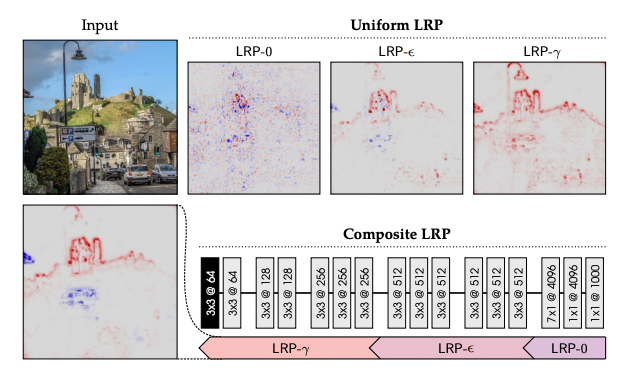
\includegraphics[width=\textwidth]{img/lrp-montavon.png}
    \end{minipage}
    \caption{Image show explanation results after different combination of rules is applied. Notice, that combining multiple rules yields visualy more coherent saliency map. According to Montavon, it is beneficial to use LRP-$0$ in the upper layers, to combat entanglement of different concepts represented by the network. LRP-$\epsilon$ in the middle layer helps to propagate only the most salient activations, while LRP-$\gamma$ in the lower layer ensures uniform relevance spread []. Image is taken from [].}
    \label{fig:lrp-montavon}
    \end{center}
% https://iphome.hhi.de/samek/pdf/MonXAI19.pdf
\end{figure}